
%% bare_jrnl_compsoc.tex
%% V1.3
%% 2007/01/11
%% by Michael Shell
%% See:
%% http://www.michaelshell.org/
%% for current contact information.
%%
%% This is a skeleton file demonstrating the use of IEEEtran.cls
%% (requires IEEEtran.cls version 1.7 or later) with an IEEE Computer
%% Society journal paper.
%%
%% Support sites:
%% http://www.michaelshell.org/tex/ieeetran/
%% http://www.ctan.org/tex-archive/macros/latex/contrib/IEEEtran/
%% and
%% http://www.ieee.org/

%%*************************************************************************
%% Legal Notice:
%% This code is offered as-is without any warranty either expressed or
%% implied; without even the implied warranty of MERCHANTABILITY or
%% FITNESS FOR A PARTICULAR PURPOSE! 
%% User assumes all risk.
%% In no event shall IEEE or any contributor to this code be liable for
%% any damages or losses, including, but not limited to, incidental,
%% consequential, or any other damages, resulting from the use or misuse
%% of any information contained here.
%%
%% All comments are the opinions of their respective authors and are not
%% necessarily endorsed by the IEEE.
%%
%% This work is distributed under the LaTeX Project Public License (LPPL)
%% ( http://www.latex-project.org/ ) version 1.3, and may be freely used,
%% distributed and modified. A copy of the LPPL, version 1.3, is included
%% in the base LaTeX documentation of all distributions of LaTeX released
%% 2003/12/01 or later.
%% Retain all contribution notices and credits.
%% ** Modified files should be clearly indicated as such, including  **
%% ** renaming them and changing author support contact information. **
%%
%% File list of work: IEEEtran.cls, IEEEtran_HOWTO.pdf, bare_adv.tex,
%%                    bare_conf.tex, bare_jrnl.tex, bare_jrnl_compsoc.tex
%%*************************************************************************

% *** Authors should verify (and, if needed, correct) their LaTeX system  ***
% *** with the testflow diagnostic prior to trusting their LaTeX platform ***
% *** with production work. IEEE's font choices can trigger bugs that do  ***
% *** not appear when using other class files.                            ***
% The testflow support page is at:
% http://www.michaelshell.org/tex/testflow/




% Note that the a4paper option is mainly intended so that authors in
% countries using A4 can easily print to A4 and see how their papers will
% look in print - the typesetting of the document will not typically be
% affected with changes in paper size (but the bottom and side margins will).
% Use the testflow package mentioned above to verify correct handling of
% both paper sizes by the user's LaTeX system.
%
% Also note that the "draftcls" or "draftclsnofoot", not "draft", option
% should be used if it is desired that the figures are to be displayed in
% draft mode.
%
% The Computer Society usually requires 10pt for submissions.
%\documentclass[journal,A4paper,epsfig]{IEEEtran}
%\documentclass[journal,letterpaper,epsfig]{IEEEtran}
%\documentclass[12pt,journal,letterpaper,peerreview,draftcls,onecolumn,doublespace,epsfig]{IEEEtran}

%\documentclass[journal,letterpaper,peerreview, epsfig]{IEEEtran}
\documentclass[10pt,journal,A4paper,compsoc,epsfig]{IEEEtran}
%
% If IEEEtran.cls has not been installed into the LaTeX system files,
% manually specify the path to it like:
% \documentclass[12pt,journal,compsoc]{../sty/IEEEtran}





% Some very useful LaTeX packages include:
% (uncomment the ones you want to load)


% *** MISC UTILITY PACKAGES ***
%
%\usepackage{ifpdf}
% Heiko Oberdiek's ifpdf.sty is very useful if you need conditional
% compilation based on whether the output is pdf or dvi.
% usage:
% \ifpdf
%   % pdf code
% \else
%   % dvi code
% \fi
% The latest version of ifpdf.sty can be obtained from:
% http://www.ctan.org/tex-archive/macros/latex/contrib/oberdiek/
% Also, note that IEEEtran.cls V1.7 and later provides a builtin
% \ifCLASSINFOpdf conditional that works the same way.
% When switching from latex to pdflatex and vice-versa, the compiler may
% have to be run twice to clear warning/error messages.





% *** CITATION PACKAGES ***
%
\ifCLASSOPTIONcompsoc
  % IEEE Computer Society needs nocompress option
  % requires cite.sty v4.0 or later (November 2003)
   \usepackage[nocompress]{cite}
\else
  % normal IEEE
   \usepackage{cite}
\fi
% cite.sty was written by Donald Arseneau
% V1.6 and later of IEEEtran pre-defines the format of the cite.sty package
% \cite{} output to follow that of IEEE. Loading the cite package will
% result in citation numbers being automatically sorted and properly
% "compressed/ranged". e.g., [1], [9], [2], [7], [5], [6] without using
% cite.sty will become [1], [2], [5]--[7], [9] using cite.sty. cite.sty's
% \cite will automatically add leading space, if needed. Use cite.sty's
% noadjust option (cite.sty V3.8 and later) if you want to turn this off.
% cite.sty is already installed on most LaTeX systems. Be sure and use
% version 4.0 (2003-05-27) and later if using hyperref.sty. cite.sty does
% not currently provide for hyperlinked citations.
% The latest version can be obtained at:
% http://www.ctan.org/tex-archive/macros/latex/contrib/cite/
% The documentation is contained in the cite.sty file itself.
%
% Note that some packages require special options to format as the Computer
% Society requires. In particular, Computer Society  papers do not use
% compressed citation ranges as is done in typical IEEE papers
% (e.g., [1]-[4]). Instead, they list every citation separately in order
% (e.g., [1], [2], [3], [4]). To get the latter we need to load the cite
% package with the nocompress option which is supported by cite.sty v4.0
% and later. Note also the use of a CLASSOPTION conditional provided by
% IEEEtran.cls V1.7 and later.





% *** GRAPHICS RELATED PACKAGES ***
%
\ifCLASSINFOpdf
  \usepackage[pdftex]{graphicx}
%  % declare the path(s) where your graphic files are
   \graphicspath{{./}}
%  % and their extensions so you won't have to specify these with
%  % every instance of \includegraphics
   \DeclareGraphicsExtensions{.pdf,.jpg,.png,.tif}
    \usepackage[pdftex]{subfig}
\else
  % or other class option (dvipsone, dvipdf, if not using dvips). graphicx
  % will default to the driver specified in the system graphics.cfg if no
  % driver is specified.
   \usepackage[dvips]{graphicx}
  % declare the path(s) where your graphic files are
   \graphicspath{{./}}
  % and their extensions so you won't have to specify these with
  % every instance of \includegraphics
   \DeclareGraphicsExtensions{.eps}
\fi
% graphicx was written by David Carlisle and Sebastian Rahtz. It is
% required if you want graphics, photos, etc. graphicx.sty is already
% installed on most LaTeX systems. The latest version and documentation can
% be obtained at: 
% http://www.ctan.org/tex-archive/macros/latex/required/graphics/
% Another good source of documentation is "Using Imported Graphics in
% LaTeX2e" by Keith Reckdahl which can be found as epslatex.ps or
% epslatex.pdf at: http://www.ctan.org/tex-archive/info/
%
% latex, and pdflatex in dvi mode, support graphics in encapsulated
% postscript (.eps) format. pdflatex in pdf mode supports graphics
% in .pdf, .jpeg, .png and .mps (metapost) formats. Users should ensure
% that all non-photo figures use a vector format (.eps, .pdf, .mps) and
% not a bitmapped formats (.jpeg, .png). IEEE frowns on bitmapped formats
% which can result in "jaggedy"/blurry rendering of lines and letters as
% well as large increases in file sizes.
%
% You can find documentation about the pdfTeX application at:
% http://www.tug.org/applications/pdftex





% *** MATH PACKAGES ***
%
\usepackage[cmex10]{amsmath}
\usepackage{amssymb, amsbsy,bm}
% A popular package from the American Mathematical Society that provides
% many useful and powerful commands for dealing with mathematics. If using
% it, be sure to load this package with the cmex10 option to ensure that
% only type 1 fonts will utilized at all point sizes. Without this option,
% it is possible that some math symbols, particularly those within
% footnotes, will be rendered in bitmap form which will result in a
% document that can not be IEEE Xplore compliant!
%
% Also, note that the amsmath package sets \interdisplaylinepenalty to 10000
% thus preventing page breaks from occurring within multiline equations. Use:
\interdisplaylinepenalty=2500
% after loading amsmath to restore such page breaks as IEEEtran.cls normally
% does. amsmath.sty is already installed on most LaTeX systems. The latest
% version and documentation can be obtained at:
% http://www.ctan.org/tex-archive/macros/latex/required/amslatex/math/





% *** SPECIALIZED LIST PACKAGES ***
%
\usepackage{algorithm}
\usepackage[noend]{algorithmic}
% algorithmic.sty was written by Peter Williams and Rogerio Brito.
% This package provides an algorithmic environment fo describing algorithms.
% You can use the algorithmic environment in-text or within a figure
% environment to provide for a floating algorithm. Do NOT use the algorithm
% floating environment provided by algorithm.sty (by the same authors) or
% algorithm2e.sty (by Christophe Fiorio) as IEEE does not use dedicated
% algorithm float types and packages that provide these will not provide
% correct IEEE style captions. The latest version and documentation of
% algorithmic.sty can be obtained at:
% http://www.ctan.org/tex-archive/macros/latex/contrib/algorithms/
% There is also a support site at:
% http://algorithms.berlios.de/index.html
% Also of interest may be the (relatively newer and more customizable)
% algorithmicx.sty package by Szasz Janos:
% http://www.ctan.org/tex-archive/macros/latex/contrib/algorithmicx/




% *** ALIGNMENT PACKAGES ***
%
\usepackage{array}
% Frank Mittelbach's and David Carlisle's array.sty patches and improves
% the standard LaTeX2e array and tabular environments to provide better
% appearance and additional user controls. As the default LaTeX2e table
% generation code is lacking to the point of almost being broken with
% respect to the quality of the end results, all users are strongly
% advised to use an enhanced (at the very least that provided by array.sty)
% set of table tools. array.sty is already installed on most systems. The
% latest version and documentation can be obtained at:
% http://www.ctan.org/tex-archive/macros/latex/required/tools/


%\usepackage{mdwmath}
%\usepackage{mdwtab}
% Also highly recommended is Mark Wooding's extremely powerful MDW tools,
% especially mdwmath.sty and mdwtab.sty which are used to format equations
% and tables, respectively. The MDWtools set is already installed on most
% LaTeX systems. The lastest version and documentation is available at:
% http://www.ctan.org/tex-archive/macros/latex/contrib/mdwtools/


% IEEEtran contains the IEEEeqnarray family of commands that can be used to
% generate multiline equations as well as matrices, tables, etc., of high
% quality.


%\usepackage{eqparbox}
% Also of notable interest is Scott Pakin's eqparbox package for creating
% (automatically sized) equal width boxes - aka "natural width parboxes".
% Available at:
% http://www.ctan.org/tex-archive/macros/latex/contrib/eqparbox/





% *** SUBFIGURE PACKAGES ***
%\ifCLASSOPTIONcompsoc
%\usepackage[tight,normalsize,sf,SF]{subfigure}
%\else
%\usepackage[tight,footnotesize]{subfigure}
%\fi
% subfigure.sty was written by Steven Douglas Cochran. This package makes it
% easy to put subfigures in your figures. e.g., "Figure 1a and 1b". For IEEE
% work, it is a good idea to load it with the tight package option to reduce
% the amount of white space around the subfigures. Computer Society papers
% use a larger font and \sffamily font for their captions, hence the
% additional options needed under compsoc mode. subfigure.sty is already
% installed on most LaTeX systems. The latest version and documentation can
% be obtained at:
% http://www.ctan.org/tex-archive/obsolete/macros/latex/contrib/subfigure/
% subfigure.sty has been superceeded by subfig.sty.


%\ifCLASSOPTIONcompsoc
% \usepackage[caption=false]{caption}
% \usepackage[font=normalsize,labelfont=sf,textfont=sf]{subfig}
%\else
%  \usepackage[caption=false]{caption}
%  \usepackage[font=footnotesize]{subfig}
%\fi
% subfig.sty, also written by Steven Douglas Cochran, is the modern
% replacement for subfigure.sty. However, subfig.sty requires and
% automatically loads Axel Sommerfeldt's caption.sty which will override
% IEEEtran.cls handling of captions and this will result in nonIEEE style
% figure/table captions. To prevent this problem, be sure and preload
% caption.sty with its "caption=false" package option. This is will preserve
% IEEEtran.cls handing of captions. Version 1.3 (2005/06/28) and later 
% (recommended due to many improvements over 1.2) of subfig.sty supports
% the caption=false option directly:
%\ifCLASSOPTIONcompsoc
 % \usepackage[caption=false,font=normalsize,labelfont=sf,textfont=sf]{subfig}
%\else
%  \usepackage[caption=false,font=footnotesize]{subfig}
%\fi
%
% The latest version and documentation can be obtained at:
% http://www.ctan.org/tex-archive/macros/latex/contrib/subfig/
% The latest version and documentation of caption.sty can be obtained at:
% http://www.ctan.org/tex-archive/macros/latex/contrib/caption/


%\usepackage[nomarkers]{endfloat}

% *** FLOAT PACKAGES ***
%
%\usepackage{fixltx2e}
% fixltx2e, the successor to the earlier fix2col.sty, was written by
% Frank Mittelbach and David Carlisle. This package corrects a few problems
% in the LaTeX2e kernel, the most notable of which is that in current
% LaTeX2e releases, the ordering of single and double column floats is not
% guaranteed to be preserved. Thus, an unpatched LaTeX2e can allow a
% single column figure to be placed prior to an earlier double column
% figure. The latest version and documentation can be found at:
% http://www.ctan.org/tex-archive/macros/latex/base/



\usepackage{stfloats}
% stfloats.sty was written by Sigitas Tolusis. This package gives LaTeX2e
% the ability to do double column floats at the bottom of the page as well
% as the top. (e.g., "\begin{figure*}[!b]" is not normally possible in
% LaTeX2e). It also provides a command:
%\fnbelowfloat
% to enable the placement of footnotes below bottom floats (the standard
% LaTeX2e kernel puts them above bottom floats). This is an invasive package
% which rewrites many portions of the LaTeX2e float routines. It may not work
% with other packages that modify the LaTeX2e float routines. The latest
% version and documentation can be obtained at:
% http://www.ctan.org/tex-archive/macros/latex/contrib/sttools/
% Documentation is contained in the stfloats.sty comments as well as in the
% presfull.pdf file. Do not use the stfloats baselinefloat ability as IEEE
% does not allow \baselineskip to stretch. Authors submitting work to the
% IEEE should note that IEEE rarely uses double column equations and
% that authors should try to avoid such use. Do not be tempted to use the
% cuted.sty or midfloat.sty packages (also by Sigitas Tolusis) as IEEE does
% not format its papers in such ways.




%\ifCLASSOPTIONcaptionsoff
%  \usepackage[nomarkers]{endfloat}
% \let\MYoriglatexcaption\caption
% \renewcommand{\caption}[2][\relax]{\MYoriglatexcaption[#2]{#2}}
%\fi
% endfloat.sty was written by James Darrell McCauley and Jeff Goldberg.
% This package may be useful when used in conjunction with IEEEtran.cls'
% captionsoff option. Some IEEE journals/societies require that submissions
% have lists of figures/tables at the end of the paper and that
% figures/tables without any captions are placed on a page by themselves at
% the end of the document. If needed, the draftcls IEEEtran class option or
% \CLASSINPUTbaselinestretch interface can be used to increase the line
% spacing as well. Be sure and use the nomarkers option of endfloat to
% prevent endfloat from "marking" where the figures would have been placed
% in the text. The two hack lines of code above are a slight modification of
% that suggested by in the endfloat docs (section 8.3.1) to ensure that
% the full captions always appear in the list of figures/tables - even if
% the user used the short optional argument of \caption[]{}.
% IEEE papers do not typically make use of \caption[]'s optional argument,
% so this should not be an issue. A similar trick can be used to disable
% captions of packages such as subfig.sty that lack options to turn off
% the subcaptions:
% For subfig.sty:
% \let\MYorigsubfloat\subfloat
% \renewcommand{\subfloat}[2][\relax]{\MYorigsubfloat[]{#2}}
% For subfigure.sty:
% \let\MYorigsubfigure\subfigure
% \renewcommand{\subfigure}[2][\relax]{\MYorigsubfigure[]{#2}}
% However, the above trick will not work if both optional arguments of
% the \subfloat/subfig command are used. Furthermore, there needs to be a
% description of each subfigure *somewhere* and endfloat does not add
% subfigure captions to its list of figures. Thus, the best approach is to
% avoid the use of subfigure captions (many IEEE journals avoid them anyway)
% and instead reference/explain all the subfigures within the main caption.
% The latest version of endfloat.sty and its documentation can obtained at:
% http://www.ctan.org/tex-archive/macros/latex/contrib/endfloat/
%
% The IEEEtran \ifCLASSOPTIONcaptionsoff conditional can also be used
% later in the document, say, to conditionally put the References on a 
% page by themselves.




\usepackage{algorithm}
\usepackage{algorithmic}

% *** PDF, URL AND HYPERLINK PACKAGES ***
%
\usepackage{url}
% url.sty was written by Donald Arseneau. It provides better support for
% handling and breaking URLs. url.sty is already installed on most LaTeX
% systems. The latest version can be obtained at:
% http://www.ctan.org/tex-archive/macros/latex/contrib/misc/
% Read the url.sty source comments for usage information. Basically,
% \url{my_url_here}.




% *** Do not adjust lengths that control margins, column widths, etc. ***
% *** Do not use packages that alter fonts (such as pslatex).         ***
% There should be no need to do such things with IEEEtran.cls V1.6 and later.
% (Unless specifically asked to do so by the journal or conference you plan
% to submit to, of course. )


% correct bad hyphenation here
\hyphenation{op-tical net-works semi-conduc-tor}

%\newcommand{\indicator}{1{\hskip -2.5 pt}\hbox{I} \qquad \qquad}}
\newcommand{\indicator}{1\hspace{-2.5mm}{1}}



%% Alter some LaTeX defaults for better treatment of figures:
%    % See p.105 of "TeX Unbound" for suggested values.
%    % See pp. 199-200 of Lamport's "LaTeX" book for details.
%    %   General parameters, for ALL pages:
%    \renewcommand{\topfraction}{0.9}	% max fraction of floats at top
%    \renewcommand{\bottomfraction}{0.8}	% max fraction of floats at bottom
%    %   Parameters for TEXT pages (not float pages):
%    \setcounter{topnumber}{2}
%    \setcounter{bottomnumber}{2}
%    \setcounter{totalnumber}{4}     % 2 may work better
%    \setcounter{dbltopnumber}{2}    % for 2-column pages
%    \renewcommand{\dbltopfraction}{0.9}	% fit big float above 2-col. text
%    \renewcommand{\textfraction}{0.07}	% allow minimal text w. figs
%    %   Parameters for FLOAT pages (not text pages):
%    \renewcommand{\floatpagefraction}{0.7}	% require fuller float pages
%	% N.B.: floatpagefraction MUST be less than topfraction !!
%    \renewcommand{\dblfloatpagefraction}{0.7}	% require fuller float pages

%	% remember to use [htp] or [htpb] for placement

\usepackage[export]{adjustbox}
\usepackage{pgfplots}

\begin{document}
%
% paper title
% can use linebreaks \\ within to get better formatting as desired
\title{Emotion Recognition from EEG Signals}
%
%
% author names and IEEE memberships
% note positions of commas and nonbreaking spaces ( ~ ) LaTeX will not break
% a structure at a ~ so this keeps an author's name from being broken across
% two lines.
% use \thanks{} to gain access to the first footnote area
% a separate \thanks must be used for each paragraph as LaTeX2e's \thanks
% was not built to handle multiple paragraphs
%
%
%\IEEEcompsocitemizethanks is a special \thanks that produces the bulleted
% lists the Computer Society journals use for "first footnote" author
% affiliations. Use \IEEEcompsocthanksitem which works much like \item
% for each affiliation group. When not in compsoc mode,
% \IEEEcompsocitemizethanks becomes like \thanks and
% \IEEEcompsocthanksitem becomes a line break with idention. This
% facilitates dual compilation, although admittedly the differences in the
% desired content of \author between the different types of papers makes a
% one-size-fits-all approach a daunting prospect. For instance, compsoc 
% journal papers have the author affiliations above the "Manuscript
% received ..."  text while in non-compsoc journals this is reversed. Sigh.




\author{Alessio Quercia
        \thanks{Alessio Quercia, Natural Interaction and Models for Affecting Computing Courses,  A/A 2017-2018, Universit\`{a} degli Studi di Milano, via Comelico 39/41, Milano, Italy \protect\\
% note need leading \protect in front of \\ to get a newline within \thanks as
% \\ is fragile and will error, could use \hfil\break instead.
E-mail: alessio.quercia@studenti.unimi.it}%
\thanks{}}

% note the % following the last \IEEEmembership and also \thanks - 
% these prevent an unwanted space from occurring between the last author name
% and the end of the author line. i.e., if you had this:
% 
% \author{....lastname \thanks{...} \thanks{...} }
%                     ^------------^------------^----Do not want these spaces!
%
% a space would be appended to the last name and could cause every name on that
% line to be shifted left slightly. This is one of those "LaTeX things". For
% instance, "\textbf{A} \textbf{B}" will typeset as "A B" not "AB". To get
% "AB" then you have to do: "\textbf{A}\textbf{B}"
% \thanks is no different in this regard, so shield the last } of each \thanks
% that ends a line with a % and do not let a space in before the next \thanks.
% Spaces after \IEEEmembership other than the last one are OK (and needed) as
% you are supposed to have spaces between the names. For what it is worth,
% this is a minor point as most people would not even notice if the said evil
% space somehow managed to creep in.



% The paper headers
%\markboth{IEEE Trans. on PAMI, September 5,~2011}{Boccignone and Ferraro}
%\markboth{submitted to IEEE Trans. on SMC-B}{ }
% The only time the second header will appear is for the odd numbered pages
% after the title page when using the twoside option.
% 
% *** Note that you probably will NOT want to include the author's ***
% *** name in the headers of peer review papers.                   ***
% You can use \ifCLASSOPTIONpeerreview for conditional compilation here if
% you desire.



% The publisher's ID mark at the bottom of the page is less important with
% Computer Society journal papers as those publications place the marks
% outside of the main text columns and, therefore, unlike regular IEEE
% journals, the available text space is not reduced by their presence.
% If you want to put a publisher's ID mark on the page you can do it like
% this:
%\IEEEpubid{0000--0000/00\$00.00~\copyright~2007 IEEE}
% or like this to get the Computer Society new two part style.
%\IEEEpubid{\makebox[\columnwidth]{\hfill 0000--0000/00/\$00.00~\copyright~2007 IEEE}%
%\hspace{\columnsep}\makebox[\columnwidth]{Published by the IEEE Computer Society\hfill}}
% Remember, if you use this you must call \IEEEpubidadjcol in the second
% column for its text to clear the IEEEpubid mark (Computer Society jorunal
% papers don't need this extra clearance.)


% make the title area
\maketitle


% for Computer Society papers, we must declare the abstract and index terms
% PRIOR to the title within the \IEEEcompsoctitleabstractindextext IEEEtran
% command as these need to go into the title area created by \maketitle.
%\IEEEcompsoctitleabstractindextext{%
\begin{abstract}
%\boldmath
In this paper I show classification results for emotion recognition from EEG signals, based on the method described in the article \cite{zhuang2017emotion}. This method consists in making classification and prediction using features extracted from decomposed EEG signals.

First of all, EEG signals taken from the DEAP dataset are decomposed into IMFs (Intrinsic Mode Functions) using the EMD (Empirical Mode Decomposition), then the first difference of time series, the first difference of phase and the normalized energy are extracted as features from the first IMF, the most informative one. Two disjoint sets are formed using the extracted features: a training set and a test set. Classification was made on the training set and the respective label set; then, prediction was made on the test set, to test the trained model on a different set without giving it the labels as input. Predicted values was confronted with the labels to check if the model prediction was right or wrong.
Using cross-validation, it was possible to extimate the model accuracy for a single participant in the DEAP dataset. Finally the method accuracy was computed as the mean of the accuracies computed on the single participants.



\end{abstract}




\section{Introduction}
\label{sec:introduction}


Emotions play an important role in our daily life. Indeed we use them everyday consciously or subconsciously in decision-making processes, in human interaction and for the perception of the world around us.
They are also an important factor in Human-Computer Interaction (HCI), which aims at improving the communication between humans and computers, and Affective Computing, which aims at modeling emotional interactions between humans and computers by measuring users' emotional states. 
A person can be asked to report how he is feelin while watching a video, but the subjective self-reports alone are not enough to correctly measure his emotional state, because he may answer not exactly how he is feeling. For this reason, physiological signals can be measured to help understanding the person's emotional state. Different kinds of signals can be used for this purpose: the Galvanic Skin Response (GSR), which increases linearly with a person's level of arousal, the Electromyography (EMG), which measures the frequency of muscle tension and is correlated with negatively valenced emotions, the Heart Rate (HR), which increases with negatively valenced emotions (such as fear), the Respiration Rate (RR), which measures how deep and fast the breath is and becomes irregular with more aroused emotions (such as anger), the Electroencephalography (EEG), which has a poor space resolution, but a great time resolution, that allows to study the phase changes in response to emotional stimuli \cite{zhuang2017emotion, alarcao2017emotions}.


There are many features extraction methods used to recognize emotions from EEG signals, including time domain techniques, frequency domain techniques and joint time-frequency analysis techniques. Also there are different types of features to extract from EEG signals, such as first and second difference, mean value and power (usually used in time domain techniques), or nonlinear features like fractal dimension (FD), sample entropy and nonstationary index.

I used the method described in the article \cite{zhuang2017emotion}. The method consists in the following steps:
\begin{enumerate}
\item Sampling the EEG signals each 5 seconds.
\item EEG signal samples decomposition into Intrinsic Mode Functions (IMFs) using Empirical Mode Decomposition (EMD).
\item Features extraction from the most informative IMF of the most informative channels, forming two disjoint sets, a training set and a test set. For each IMF three features are extracted: the first difference of IMF time series, the first difference of IMF's phase and the normalized energy. These three features depict the characteristics of the IMF in time, frequency and energy domain, providing multidimensional information.
\item Classification on the training set, composed by most of the extracted features, together with their respective labels.
\item Prediction on the test set, composed only by the remaining features.
\item Recognition of the results, confronting the predicted values with the respective labels to check whether the model predicted the right value or the wrong one.
\end{enumerate}

The first step is needed to obtain more samples from a single EEG signal measured on a participant watching a 60 seconds video. 
In the second step EMD is used to decompose the EEG signal sample into IMFs, which represent different frequency components of original signals, with band-limited characteristic.
In the third step three features are extracted for each IMF. The first difference of IMF time series depicts the intensity of signal change in time domain, the first difference of IMF's phase measures the change intensity in phase and the normalized energy describes the weight of current oscillation component \cite{zhuang2017emotion}.


In this paper I show the classification and prediction results obtained for emotion recognition from EEG signals using a SVM classifier based on libsvm library, with default settings and radial basis function as kernel. Model accuracy is computed for each participant in the DEAP dataset separately and finally a mean is computed to obtain the method accuracy over all the samples used.


\section{State of the art}
\label{back}

Human-Computer Interaction, Natural Interaction and Affective Computing are subject of interest of many researches. In the last years the interest on them has increased for researchers aim at improving human lifestyle quality, by improving the communication between humans and computers, since computers have an high impact on our daily life.
There are several works on emotion recognition in literature, many of which use EEG signals to recognize emotional states. The articles \cite{alarcao2017emotions, zhuang2017emotion} on which I based my project are just two examples of these works.


\section{Background}
The following two subsections briefly describe what emotions and electroencephalography are and how they can be used for emotion recognition.

\label{background}

\subsection{Emotions}
An emotion is a complex psychological state that involves three distinct components: a subjective experience, a physiological response and a behavioral or expressive response \cite{alarcao2017emotions}. Emotions are discrete and consistent responses to events with significance for the organism. These responses may include verbal, behavioral physiological and neural mechanisms.
Emotions can be represented with two different perspectives:
\begin{itemize}
\item The \textit{categorial perspective}, which indicates that emotions have evolved through natural selection. According to this perspective there are some basic inherited emotions, for example Plutchik proposed eight basic emotions: anger, fear, sadness, disgust, surprise, curiosity, acceptance and joy.
\item The \textit{dimensional perspective} (based on cognition), which sees the emotions mapped into the Valence, Arousal and Dominance (VAD) dimensions. Valence represents how positive is the feeling and varies from very negative to very positive; Arousal (also called Activation) indicates the level of excitement and varies from states like sleepy to excited; and Dominance corresponds to the strength of the emotion.
\end{itemize}

\subsection{Electroencephalography (EEG)}
EEG is a medical imaging technique that reads the scalp electrical activity generated by brain structures, i.e., it measures voltage fluctuations resulting from ionic current flows within the neurons of the brain \cite{alarcao2017emotions}.

The cortex, the largest part of the human brain, is divided into four lobes:
\begin{itemize}
\item the frontal lobe, responsible for the conscious thought;
\item the temporal lobe, responsible for the senses of smell and sound, and the processes of complex stimuli such as faces and scenes;
\item the parietal lobe, responsible for integrating sensory information from various senses and for the manipulation of objects;
\item the occipital lobe, responsible for the sense of sight.
\end{itemize}

The signals observed with the EEG can be divided into specific ranges:
\begin{itemize}
\item the delta waves (1-4 Hz), associated with the unconscious mind;
\item the theta waves (4-7 Hz), associated with the subconscious mind;
\item the alpha waves (8-13 Hz), associated to a relaxed mental state;
\item the beta waves (13-30 Hz), related to an active state of mind;
\item the gamma waves (>30 Hz), associated with an hyper brain activity.
\end{itemize}

There are two main areas of the brain correlated with emotional activity: the \textit{amygdala} (located close to the \textit{hippocampus}, in the frontal portion of the temporal lobe) and the pre-frontal cortex (part of the frontal lobe).
The frontal and parietal lobes are the most informative about the emotional states, while the alpha, gamma and beta appear to be the most discriminative \cite{alarcao2017emotions}.


\section{Theoretical model}
 \label{model}
 
\subsection{Dataset}
The DEAP dataset consists of two parts:
\begin{enumerate}
\item The ratings from an online self-assessment where 120 one-minute extracts of music videos were each rated by 14-16 volunteers based on arousal, valence and dominance.
\item The participant ratings, physiological recordings and face video of an experiment where 32 volunteers watched a subset of 40 of the above music videos. EEG and physiological signals were recorded and each participant also rated the videos as above. For 22 participants frontal face video was also recorded.
\end{enumerate}

I used the preprocessed data contained in the second part, which consists of 32 files, corresponding to the 32 experiment's participants. These files contain a downsampled (to 128Hz), preprocessed and segmented version of the original data.
Each participant file contains two arrays, as shown in the Table \ref{table_dataset}.


%\vspace*{-3pt}
\begin{table}
\centering
\begin{tabular}{l l l}
Array name & Array shape & Array contents \\
\hline
\noalign{\medskip}
data & 40 x 40 x 8064 & video/trial x channel x data \\
\noalign{\medskip}
labels & 40 x 4 & \parbox[t]{4cm}{video/trial x label (valence, \\ arousal, dominance, liking)} \\
\noalign{\smallskip}
\hline
\end{tabular}
\caption{DEAP dataset.}
\label{table_dataset}
\end{table}%


\subsection{Sampling from the dataset}
The preprocessed EEG signals in the DEAP dataset have been sampled each 5 seconds to have bigger training and test sets. Indeed splitting the signals each 5 seconds results in having 12 samples per video, each containing 40 different signals, corresponding to 40 different channels. Repeating this for all the 40 videos proposed to each participant in the dataset, it was possible to have 480 samples per participant. The training set was formed using 468 samples, corresponding to 39 videos, and the respective labels (repeated for the 12 split samples); while the test set was formed using 12 samples, corresponding to the remaining video.


\subsection{Empirical Mode Decomposition (EMD)}

Each EEG signal sample (from here on just `sample') is decomposed into a set of Intrinsic Mode Functions (IMFs) by Empirical Mode Decomposition (EMD). Each IMF represents different frequency components of original signals.

For input signal $x(t)$, the EMD process is:
\begin{enumerate}
\item Set $h(t) = x(t)$ and $h_{old}(t) = h(t)$.

\item Get local maximum and minimum of $h_{old}(t)$.

\item Interpolate the local maximum and minimum with cubic spline function and get upper envelope $e_{max}(t)$ and and lower envelope $e_{min}(t)$.

\item Calculate the mean value of the upper and lower envelope as
\begin{equation}
m(t) = \frac{e_{min}(t) + e_{max}(t)}{2}.
\end{equation}

\item Subtract $h_{old}(t)$ with $m(t)$:
\begin{equation}
h_{new}(t) = h_{old} - m(t).
\end{equation}
If $h_{new}(t)$ satisfies the following two conditions:
\begin{enumerate}
\item during the whole data set, the number of extreme points and the number of zero crossing must be either equal or differ at most by one;
\item at each point, the mean value calculated from the upper and lower envelope must be zero;
then the first IMF component $imf_1$ is gotten; otherwise, set $h_{old}(t) = h_{new}(t)$ and go to step (2), repeating steps (2)-(5) until $h_{new}(t)$ satisfies the two conditions of IMF.
Finally $imf_1$ is gotten as
\begin{equation}
imf_1 = h_{new}(t).
\end{equation}
\end{enumerate}

\item If $imf_n$ is gotten, set $h_{old}$ as
\begin{equation}
h_{old}(t) = h_{old}(t) - imf_n.
\end{equation}
Then go to step (2) and repeat steps (2)-(5) to get $imf_{n+1}$.
\end{enumerate}

The signal $x(t)$ can be expressed as
\begin{equation}
x(t) = \sum_{n=1}^L{imf_n + r},
\end{equation}
a linear combination of IMF components and the residual part $r$ \cite{zhuang2017emotion}.

\subsection{Features extraction}
For each sample, three features have been extracted from the most informative IMF (the first) of the most (8 channels) informative electrodes (Fp1, Fp2, F7, F8, T7, T8, P7, and P8). Indeed 24 features for each sample were collected.
The three features extracted for the first imf of each of the above mentioned channels are the following \cite{zhuang2017emotion}
\begin{enumerate}
\item \textit{First difference of IMF time series}, which depicts the intensity of signal change in time domain. For an IMF component with $N$ points, IMF$\{imf_1, imf_2, ..., imf_N\}$, it can be computed as follows:
\begin{equation}
D_t = \frac{1}{N-1}\sum_{n=1}^{N-1}{|imf(n+1) - imf(n)|}.
\end{equation}

\item \textit{First difference of IMF's phase}, which reveals the change intensity of phase and represents the physical meaning of instantaneous frequency. For an $N$-point IMF, IMF$\{imf_1, imf_2, ..., imf_N\}$, Hilbert transform is applied to it, obtainig the analytic signal $z(n)$:
\begin{equation}
z(n) = x(n) + jy(n).
\end{equation}

An equivalent way of representing the analytic signal is:
\begin{equation}
z(n) = A(n) + e^{j\varphi(n)},
\end{equation}
where $A(n) = \sqrt{x(n)^2 - y(n)^2}$ is the amplitude of $z(n)$ and $\varphi(n) = arctan(y(n)/x(n)$ is the instantaneous phase.

Finally, the first difference of IMF's phase can be computed as follows:
\begin{equation}
D_p = \frac{1}{N-1}\sum_{n=1}^{N-1}{|\varphi(n+1) - \varphi(n)|}
\end{equation}

\item \textit{Normalized energy of IMF}, which describes the weight of current oscillation component. For an $N$-point IMF, IMF$\{imf_1, imf_2, ..., imf_N\}$, it can be computed as follows:
\begin{equation}
E_{norm} = \frac{\sum_{n=1}^N{imf^2(n)}}{\sum_{n=1}^N{s^2(n)}},
\end{equation}
where $s(n)$ is the original EEG signal.
\end{enumerate}.


\subsection{Classification and prediction}

Once extracted the features from the EEG signals and created a training set and a test set, I fed the first one into a SVM classifier, using standard parameters and the radial basis function as kernel, and trained it. Then I used the trained model to predict emotional states using the test set as input.

Given a training set of instance-label pairs ($x_i$, $y_i$), $i= 1, ..., l$ where $x_i \in \mathcal{R}^n$ and  $y_i \in \{-1, 1\}^l$, a SVM requires the solution of the following optimization problem:
\begin{equation}
\min_{w,b,\xi}{\frac{1}{2}w^Tw + \mathcal{C}\sum_{i=1}^l{\xi_i}}
\end{equation}
subject to
\begin{eqnarray}
y_i(w^T\phi(x_i)+b)\geq 1-\xi_i, \\
\xi_i \geq 0.
\end{eqnarray}
where $\mathcal{C} > 0$ is the penalty parameter of the error term. The training vectors $x_i$ are mapped into a higher (maybe infinite) dimentional space by the function $\phi$. SVM finds a linear separating hyperplane with the maximal margin in this higher dimentional space \cite{hsu2003practical}.

A Support Vector Machine (SVM) is a supervised learning model with an associated learning algorithm that analyze data used for classification and regression analysis. Given a set of training examples, each one marked as belonging to one or the other of two categories, a SVM training algorithm builds a model that assigns new examples to one category or the other, making it a non-probabilistic binary linear classifier.
A support vector machine constructs a hyperplane or set of hyperplanes	 in a high- or infinite-dimensional space, which can be used for classification, regression, or other tasks like outliers detection.

It often happens that the sets to discriminate are not linearly separable. SVMs can efficiently perform a non-linear classification using the \textit{kernel trick}, implicitly mapping their inputs from finite-dimensional space into higher dimentional features spaces. The kernel trick consists of observing that many machine learning algorithms can be written exclusively in terms of dot products between examples. For example:
\begin{equation}
w^Tx + b = b + \sum_{i=1}^m {\alpha_ix^Tx^{(i)}}
\end{equation}
where $x^{(i)}$ is a training example and $\alpha$ is a vector of coefficients. Rewriting the learning algorithm this way allows us to replace $x$ by the output of a given feature function $\phi(x)$ and the dot product with a function $k(x, x^{(i)}) = \phi(x)\cdot\phi(x^{(i)})$, called \textit{kernel function}.

After replacing dot products with kernel evaluations, we can make classification using the function
\begin{equation}
f\big(x^{(i)}\big) = sgn\Bigg(\Bigg[\sum_{i=1}^m{\alpha_iy_ik(x_i, x^{(i)})\Bigg] - b}\Bigg)
\end{equation}
and prediction using the function
\begin{equation}
f(x) = b + \sum_{i=1}^m {\alpha_ik(x_i, x^{(i)})}.
\end{equation}
which is nonlinear with respect to $x$, but the relationship between $\phi(x)$ and $f(x)$ and the one between $\alpha$ and $f(x)$ are both linear. 
Using the kernel function means preprocessing the data by applying $\phi(x)$ to all inputs and then learning a linear model in the new transformed space.

The most commonly used kernel is the \textit{Gaussian kernel}, also called \textit{Radial Basis Function} (RBF) kernel, because its value decreases along lines in $v$ space radiating outward from $u$:
\begin{equation}
k(u, v) = \mathcal{N}(u-v; 0, \sigma^2I)
\end{equation}
where $\mathcal{N}(x; \mu, \Sigma)$ is the standard normal density.
The Gaussian kernel corresponds to a dot products in an infinite-dimensional space. We can think it as performing a kind of \textit{template matching}: a training example $x$ associated with training label $y$ becomes a template for class $y$. When a test point $x'$ is near $x$ according to Euclidean distance, the Gaussian kernel has a large response, indicating that $x'$ is very similar to $x$ template. The model then puts a large weight on the associated training label $y$ \cite{lecun2015deep}.
The radial basis kernel can be computed as follows:
\begin{equation}
k(x_i, x_j) = e^{-\gamma \|x_i - x_j\|^2}, \gamma > 0,
\end{equation}



\section{Simulations and experiments}
\label{simul}

According the method described in the article \cite{zhuang2017emotion}, I used the \textit{cross-validation} to compute the prediction accuracy for each participant, extracting features from 39 videos to form the training set, and using the remaining video to create the test set. Looping over the videos and changing each time the video to leave out for the test set, it was possible to compute 40 classifications and 40 predictions for each participant. This allowed me to compute the prediction accuracy for each participant. Then I computed the general method accuracy as the mean of the prediction accuracies.


\subsection{System architecture}
\label{arch}
I ran the simulations on my laptop, characterized by an Intel Core i7-6700HQ CPU, a Nvidia Geforce GTX 950M GPU and 8 GB RAM. The implemented algorithm for emotion recognition uses the CPU only.

\begin{figure}
\centering
\includegraphics[scale=0.6, trim=0 7cm 15cm 2cm, center]{./Fig/scheme.eps}
\caption{Method scheme.}
\label{Fig:scheme}
\end{figure}


\subsection{Implementation details}
The implementation is based on the general method scheme represented in the Figure \ref{Fig:scheme}.

The implemented algorithm also takes in consideration the \textit{cross-validation} as shown in the pseudo-code in the Algorithm 
\ref{alg1}.

I implemented the algorithm in python, importing \textit{EMD} library from \textit{PyEMD} for the Empiric Mode Decomposition, and \textit{svm} from \textit{sklearn} for the SVM classifier.
I used the SVC classifier, based on libsvm, with standard parameters and radial basis function as kernel.

\begin{algorithm}                      % enter the algorithm environment
\caption{Emotion recognition pseudo code}          % give the algorithm a caption
\label{alg1}                           % and a label for \ref{} commands later in the document
\begin{algorithmic}                    % enter the algorithmic environment
	\FOR{\textbf{each} participant in dataset}
		\STATE data = dataset[participant]['data']
		\STATE labels = dataset[participant]['labels']
		\FOR{\textbf{each} video in data}
			\STATE features\_per\_video = extract\_features(video, data)
		\ENDFOR
		\STATE leave\_out = len(data) - 1
		\WHILE{leave\_out $>=$ 0}
			\FOR{\textbf{each} video in data}
				\IF{video == leave\_out}
					\STATE \textbf{continue}
				\ENDIF
				\STATE X.append(features\_per\_video(video))
			\ENDFOR
			\STATE LABELS = ['Valence', 'Arousal']
			\FOR{\textbf{each} lab in LABELS}
				\FOR{\textbf{each} sample}
					\STATE Y = labels[video][lab]
				\ENDFOR
				\STATE training\_set = [X, Y]
				\STATE SVM.fit(training\_set)
				
				\STATE test\_set.append(features\_per\_video(leave\_out))
				\STATE SVM.predict(test\_set)
			\ENDFOR
		\ENDWHILE
	\ENDFOR
\end{algorithmic}
\end{algorithm}







\section{Results}
The emotion recognition accuracy, considering the valence and the arousal, for each participant is showed in the Table \ref{table_results}. Valence accuracy for each participant is represented in the graph in the Figure \ref{Fig:valence_accuracy}, while arousal accuracy for each participant is represented in the graph in the Figure \ref{Fig:arousal_accuracy}. 
Results for emotion recognition using the method previously described indicate that a mean model trained with 39 videos will recognize the correct emotion felt (predicting the correct label) with about 60\% accuracy. Indeed, as shown in the Figure \ref{Fig:method_accuracy}, the mean valence prediction accuracy is 59.5\%, while the mean arousal prediction accuracy is 62\%, considering all the participants in the DEAP dataset.


%\vspace*{-3pt}
\begin{table}
\centering
\begin{tabular}{c c c}
Participant & Valence Accuracy & Arousal Accuracy \\ 
\hline 
\noalign{\medskip}
1 & $42.5\%$ & $47.5\%$ \\ \noalign{\smallskip}
2 & $62.5\%$ & $57.5\%$ \\ \noalign{\smallskip}
3 & $57.5\%$ & $80\%$ \\ \noalign{\smallskip}
4 & $62.5\%$ & $57.5\%$ \\ \noalign{\smallskip}
5 & $65\%$ & $37.5\%$ \\ \noalign{\smallskip}
6 & $70\%$ & $37.5\%$ \\ \noalign{\smallskip}
7 & $55\%$ & $50\%$ \\ \noalign{\smallskip}
8 & $47.5\%$ & $55\%$ \\ \noalign{\smallskip}
9 & $67.5\%$ & $65\%$ \\ \noalign{\smallskip}
10 & $75\%$ & $60\%$ \\ \noalign{\smallskip}
11 & $25\%$ & $75\%$ \\ \noalign{\smallskip}
12 & $62.5\%$ & $82.5\%$ \\ \noalign{\smallskip}
13 & $72.5\%$ & $85\%$ \\ \noalign{\smallskip}
14 & $70\%$ & $62.5\%$ \\ \noalign{\smallskip}
15 & $65\%$ & $62.5\%$ \\ \noalign{\smallskip}
16 & $70\%$ & $65\%$ \\ \noalign{\smallskip}
17 & $47.5\%$ & $60\%$ \\ \noalign{\smallskip}
18 & $65\%$ & $57.5\%$ \\ \noalign{\smallskip}
19 & $62.5\%$ & $67.5\%$ \\ \noalign{\smallskip}
20 & $67.5\%$ & $77.5\%$ \\ \noalign{\smallskip}
21 & $52.5\%$ & $80\%$ \\ \noalign{\smallskip}
22 & $50\%$ & $62.5\%$ \\ \noalign{\smallskip}
23 & $75\%$ & $70\%$ \\ \noalign{\smallskip}
24 & $45\%$ & $82.5\%$ \\ \noalign{\smallskip}
25 & $45\%$ & $70\%$ \\ \noalign{\smallskip}
26 & $65\%$ & $32.5\%$ \\ \noalign{\smallskip}
27 & $72.5\%$ & $65\%$ \\ \noalign{\smallskip}
28 & $70\%$ & $52.5\%$ \\ \noalign{\smallskip}
29 & $50\%$ & $67.5\%$ \\ \noalign{\smallskip}
30 & $62.5\%$ & $45\%$ \\ \noalign{\smallskip}
31 & $65\%$ & $60\%$ \\ \noalign{\smallskip}
32 & $40\%$ & $57.5\%$ \\ \noalign{\smallskip}
\hline \noalign{\medskip}
Total & $59.5\%$ & $62\%$ \\ \noalign{\smallskip} \hline 
\end{tabular}
\caption{Valence and arousal accuracies for each participant. In the last row the general method accuracies for valence and arousal are indicated (computed as the mean of all the the accuracies of the same emotion).}
\label{table_results}
\end{table}%



\begin{figure}
\begin{tikzpicture}
\begin{axis}[
    axis lines = left,
    xlabel={Participants},
    ylabel={Accuracy (\%)},
    xmin=1, xmax=32,
    ymin=0, ymax=100,
]
 
\addplot[
    color=black,
    ]
    coordinates {
    (1,42.5)(2,62.5)(3,57.5)(4,62.5)(5,65)(6,70)(7,55)(8,47.5)(9,67.5)		(10,75)(11,25)(12,62.5)(13,72.5)(14,70)(15,65)(16,70)(17,47.5)			(18,65)(19,62.5)(20,67.5)(21,52.5)(22,50)(23,75)(24,45)(25,45)			(26,65)(27,72.5)(28,70)(29,50)(30,62.5)(31,65)(32,40)
    };
 
\end{axis}
\end{tikzpicture}
\caption{Valence accuracy for each participant.}
\label{Fig:valence_accuracy}
\end{figure}



\begin{figure}
\begin{tikzpicture}
\begin{axis}[
    axis lines = left,
    xlabel={Participants},
    ylabel={Accuracy (\%)},
    xmin=1, xmax=32,
    ymin=0, ymax=100,
]
 
\addplot[
    color=black,
    ]
    coordinates {
    (1,47.5)(2,57.5)(3,80)(4,57.5)(5,37.5)(6,37.5)(7,50)(8,55)(9,65)		(10,60)(11,75)(12,82.5)(13,85)(14,62.5)(15,62.5)(16,65)(17,60)			(18,57.5)(19,67.5)(20,77.5)(21,80)(22,62.5)(23,70)(24,82.5)(25,70)		(26,32.5)(27,65)(28,52.5)(29,67.5)(30,45)(31,60)(32,57.5)
    };
 
\end{axis}
\end{tikzpicture}
\caption{Arousal accuracy for each participant.}
\label{Fig:arousal_accuracy}
\end{figure}


\begin{figure}[H]
\begin{tikzpicture}[font=\small]
    \begin{axis}[
      ybar,
      bar width=20pt,
      ylabel={Accuracy (\%)},
	  ymin = 0,
	  ymax = 100,
      xtick=data,
      axis x line=bottom,
      axis y line=left,
      enlarge x limits=0.8,
      symbolic x coords={Valence, Arousal},
      xticklabel style={anchor=base,yshift=-\baselineskip},
      nodes near coords={\pgfmathprintnumber\pgfplotspointmeta\%}
    ]
      \addplot[fill=white] coordinates {
        (Valence,59.5)
        (Arousal,62)
      };
    \end{axis}
  \end{tikzpicture}

\caption{Method accuracy.}
\label{Fig:method_accuracy}
\end{figure}




\section{Conclusions}
The method proposed in the article \cite{zhuang2017emotion} has proven to be a good method for emotion recognition, even if the results I obtained are slightly different from the one obtained by the method authors. Indeed it recognizes the correct emotion with an accuracy of about 60\%, even if it can be boosted up to have an accuracy of about 70\%.


%BIBLIOGRAFIA
%stile IEEE
\bibliographystyle{IEEEtran}
%richiama i file bib necessari
\bibliography{IEEEabrv,Progetto_INMCA}


\end{document}
